%! TEX program = pdflatex

\documentclass[oneside,solution]{tmpl}

\usepackage[utf8]{inputenc}
\usepackage[english,ukrainian]{babel}
\usepackage{float}

\title{Домашня робота}
\author{Захаров Дмитро}
\studentID{МП-31}
\instructor{Ігнатович С.Ю.}
\date{\today}
\duedate{23:59 30 квітня, 2024}
\assignno{10}
\semester{Весняний семестр 2024}
\mainproblem{Множини Жулія і Мандельброта}

\begin{document}

\maketitle

% \startsolution[print]

\problem{}

\hspace{20px}\textbf{Умова.} Пограйтеся з програмами, що будують множини Жулія і Мандельброта. Для множини Жулія можна змінювати параметр і дивитися, як змінюється форма множини. Можна змінювати кількість кроків і стежити, як уточнюється рисунок. Для множини Мандельброта можна зображати в більшому масштабі цікаві фрагменти. Крім того, можна спробувати погратися з палітрами.

Завантажте в гугл-клас найкращі з рисунків, які у Вас вийшли. Не забудьте додати коментарі.

\textbf{Розв'язання.} 

\textbf{Множина Жулія.} Тут я експериментував з палітрами та параметром $c$. З палітрами, я вирішив просто перебрати усі можливі :) Знизу, код і картинки.

\begin{lstlisting}[language=Python]
import numpy as np
import matplotlib.pyplot as plt
from matplotlib import colormaps

def julia(xmin, xmax, Nx, ymin, ymax, Ny, steps=150):
    x = np.linspace(xmin,xmax,Nx)
    y = np.linspace(ymin,ymax,Ny)
    z = x[np.newaxis,:] + 1j*y[:,np.newaxis]
    c = 0.12 + 1j*0.62
    image = np.zeros((Nx, Ny)) 
    M = max(2,abs(c))
    
    for k in range(steps):
        z = z*z + c
        mask = (np.abs(z) > M) 
        image[mask] = k + 5
        z[mask] = np.nan
    return image[::-1,:] 
      
fig, ax = plt.subplots()
ax.set_aspect('equal')
ax.grid()

N = 2000
xmin,xmax = -1.5,1.5
ymin,ymax = -1,1

jul = julia(xmin,xmax,N,ymin,ymax,N)
for cmp in list(colormaps):
    ax.imshow(jul, 
            cmap=cmp, 
            interpolation='none',
            extent=[xmin,xmax,ymin,ymax])
    plt.tight_layout()
    fig.savefig(f'julia_{cmp}.jpg', dpi=1000)
\end{lstlisting}

\begin{figure}
    \centering
    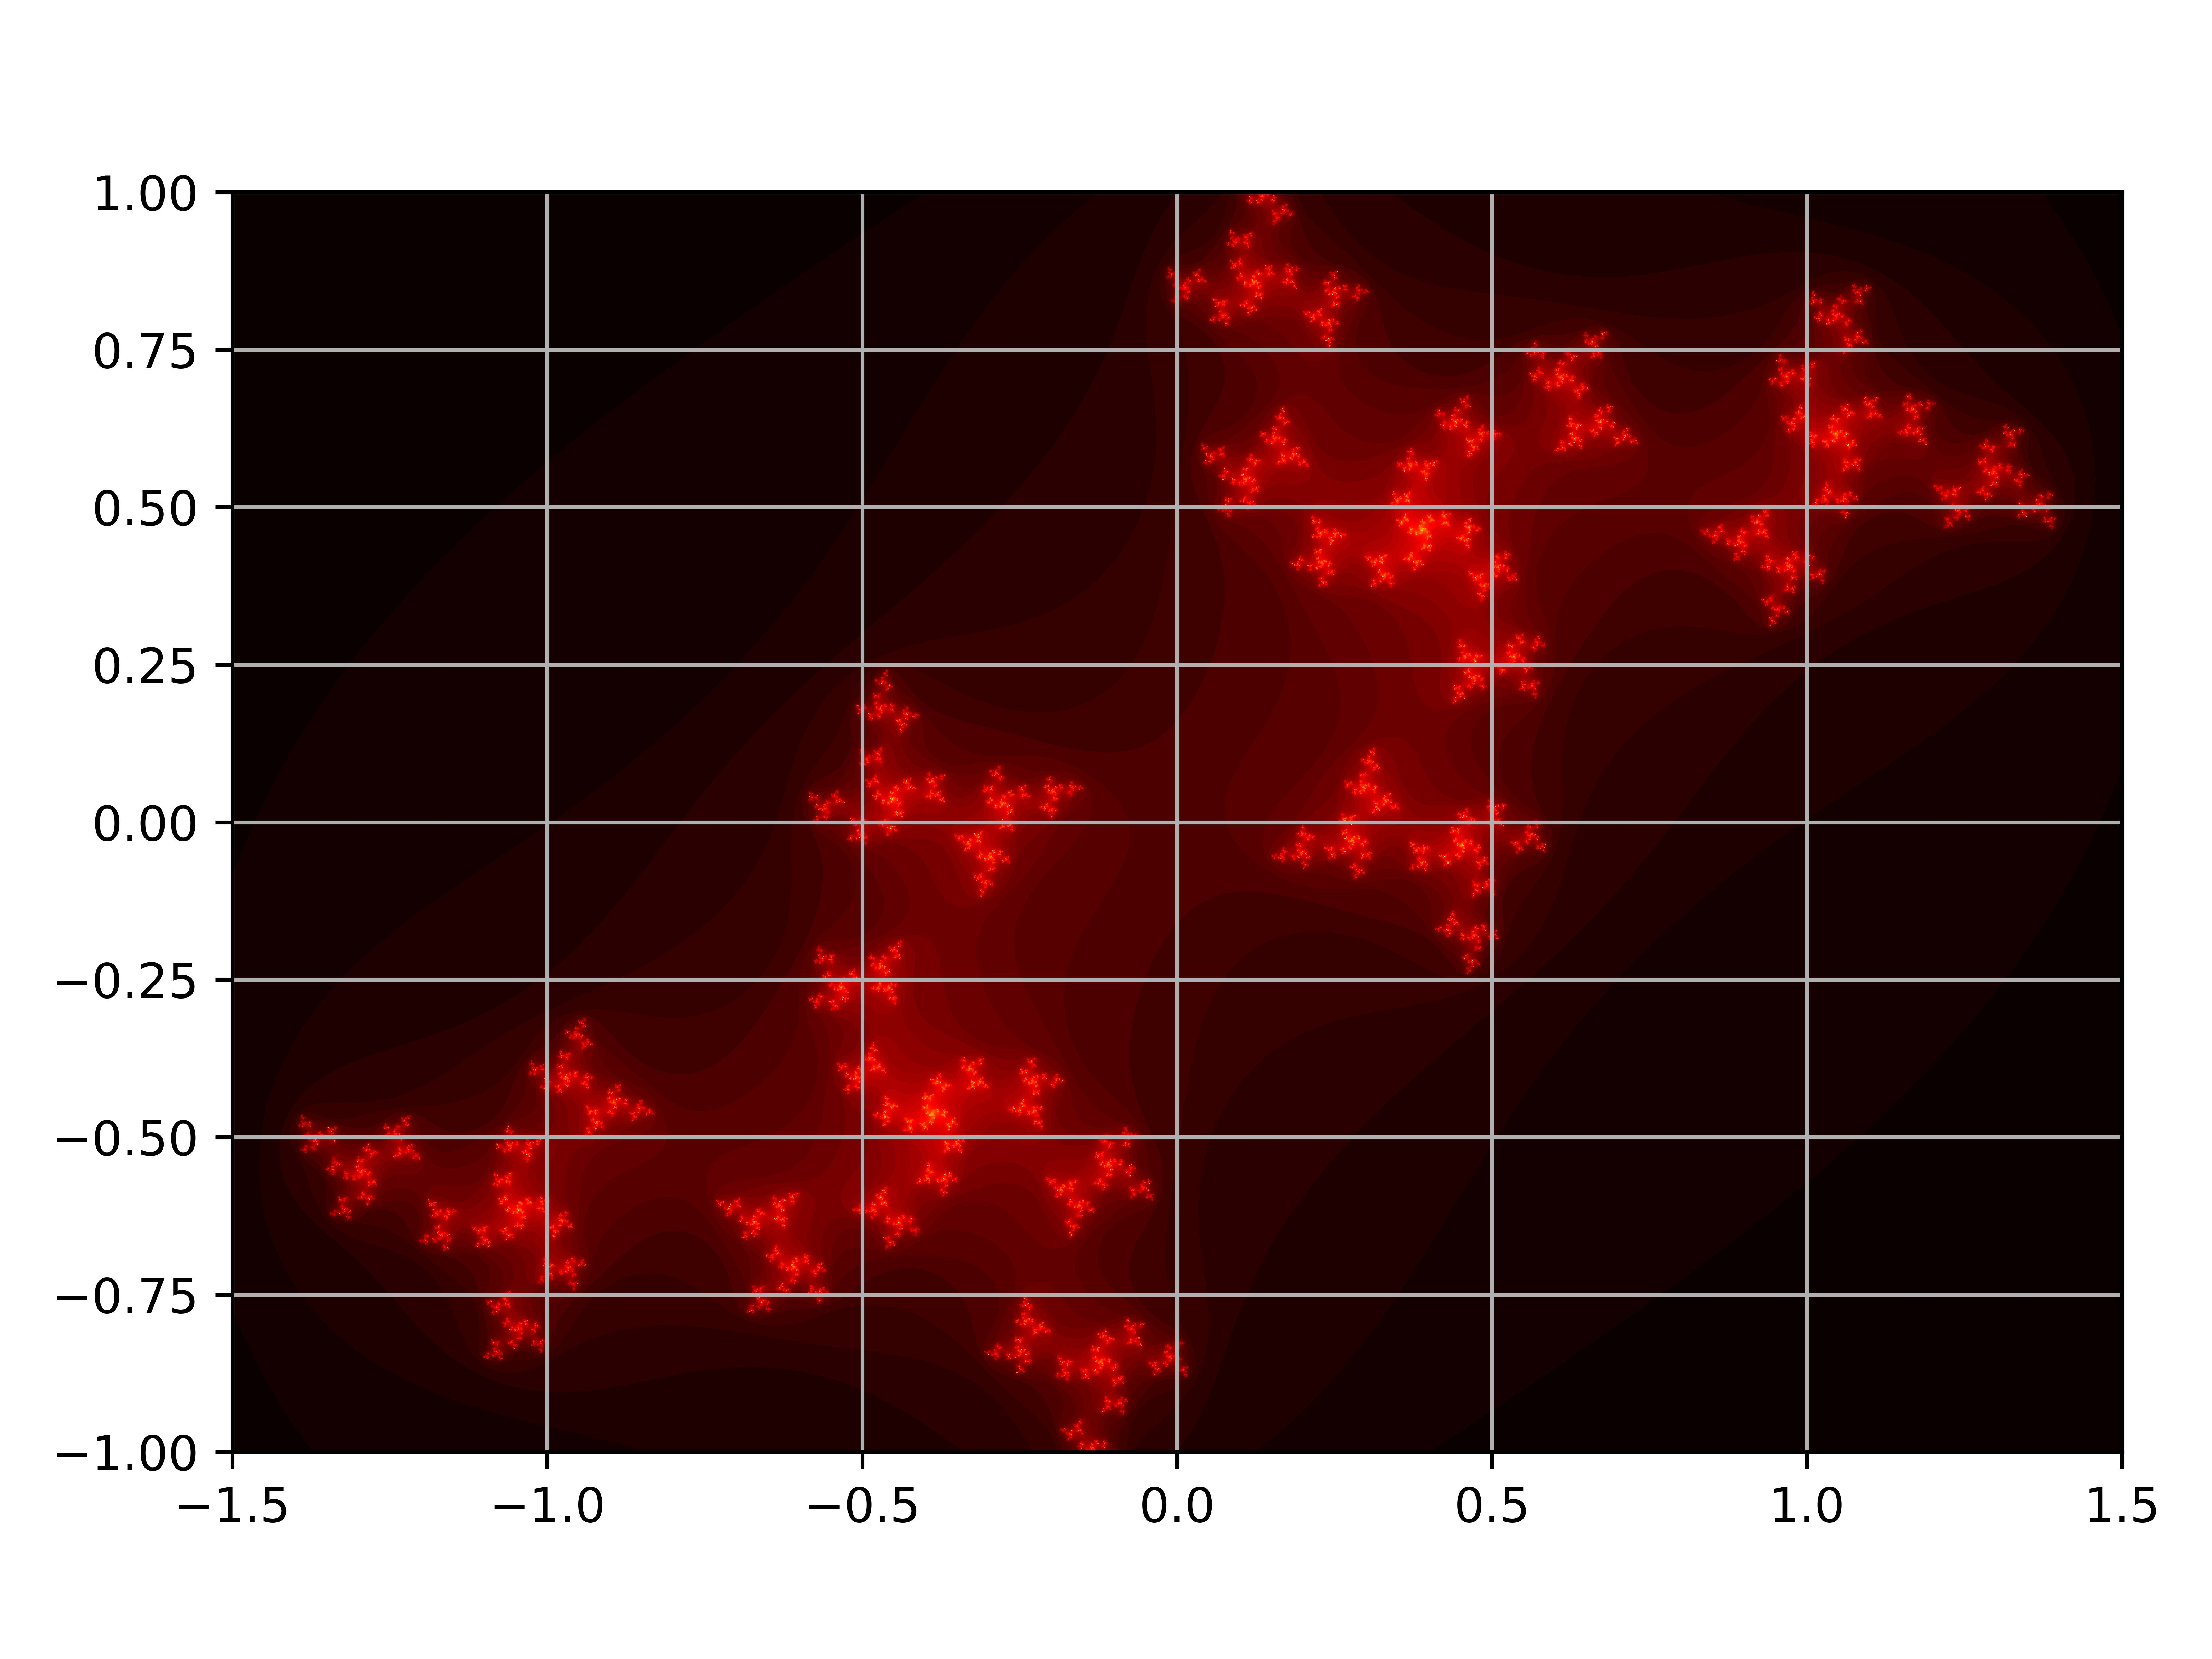
\includegraphics[width=\textwidth]{images/hw_10/julia_1.jpg}
    \caption{Множина Жулія з \texttt{gist\_heat}. Доволі цікаві теплі кольори.}
    \label{fig:1}
\end{figure}

\begin{figure}
    \centering
    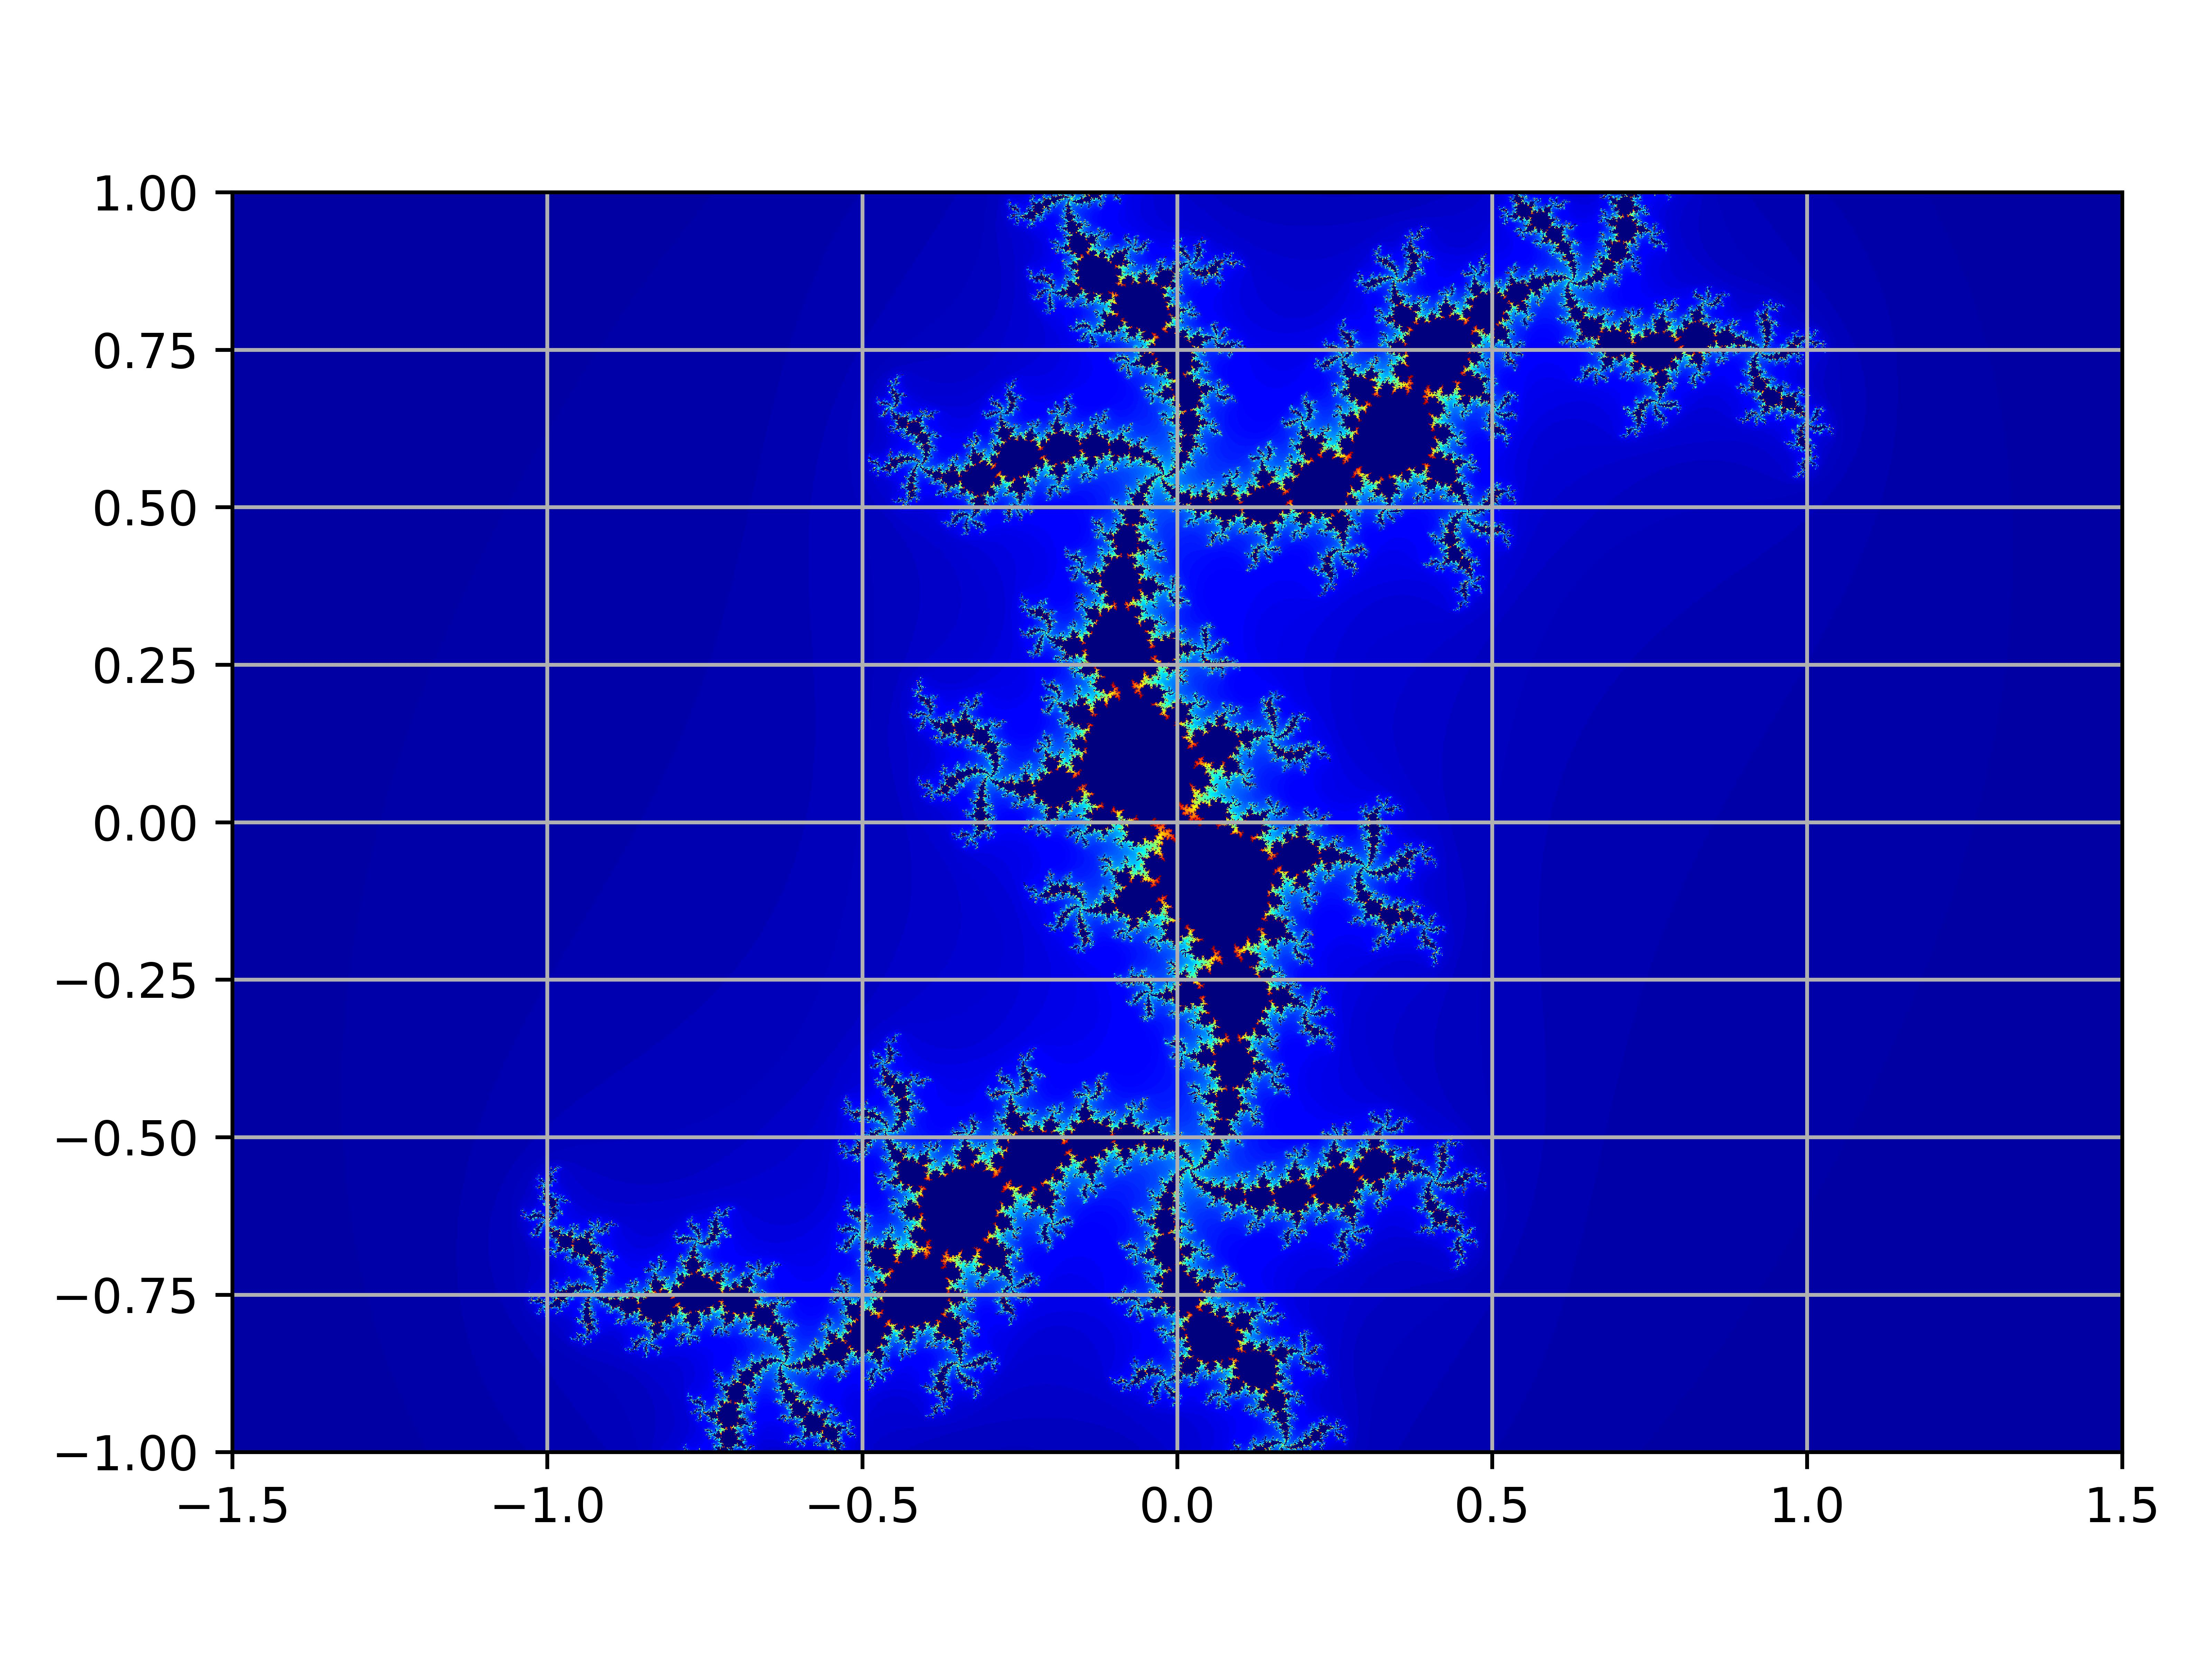
\includegraphics[width=\textwidth]{images/hw_10/julia_2.jpg}
    \caption{Множина Жулія з \texttt{brg}. Тут навпаки -- кольори дуже холодні.}
    \label{fig:2}
\end{figure}

\begin{figure}
    \centering
    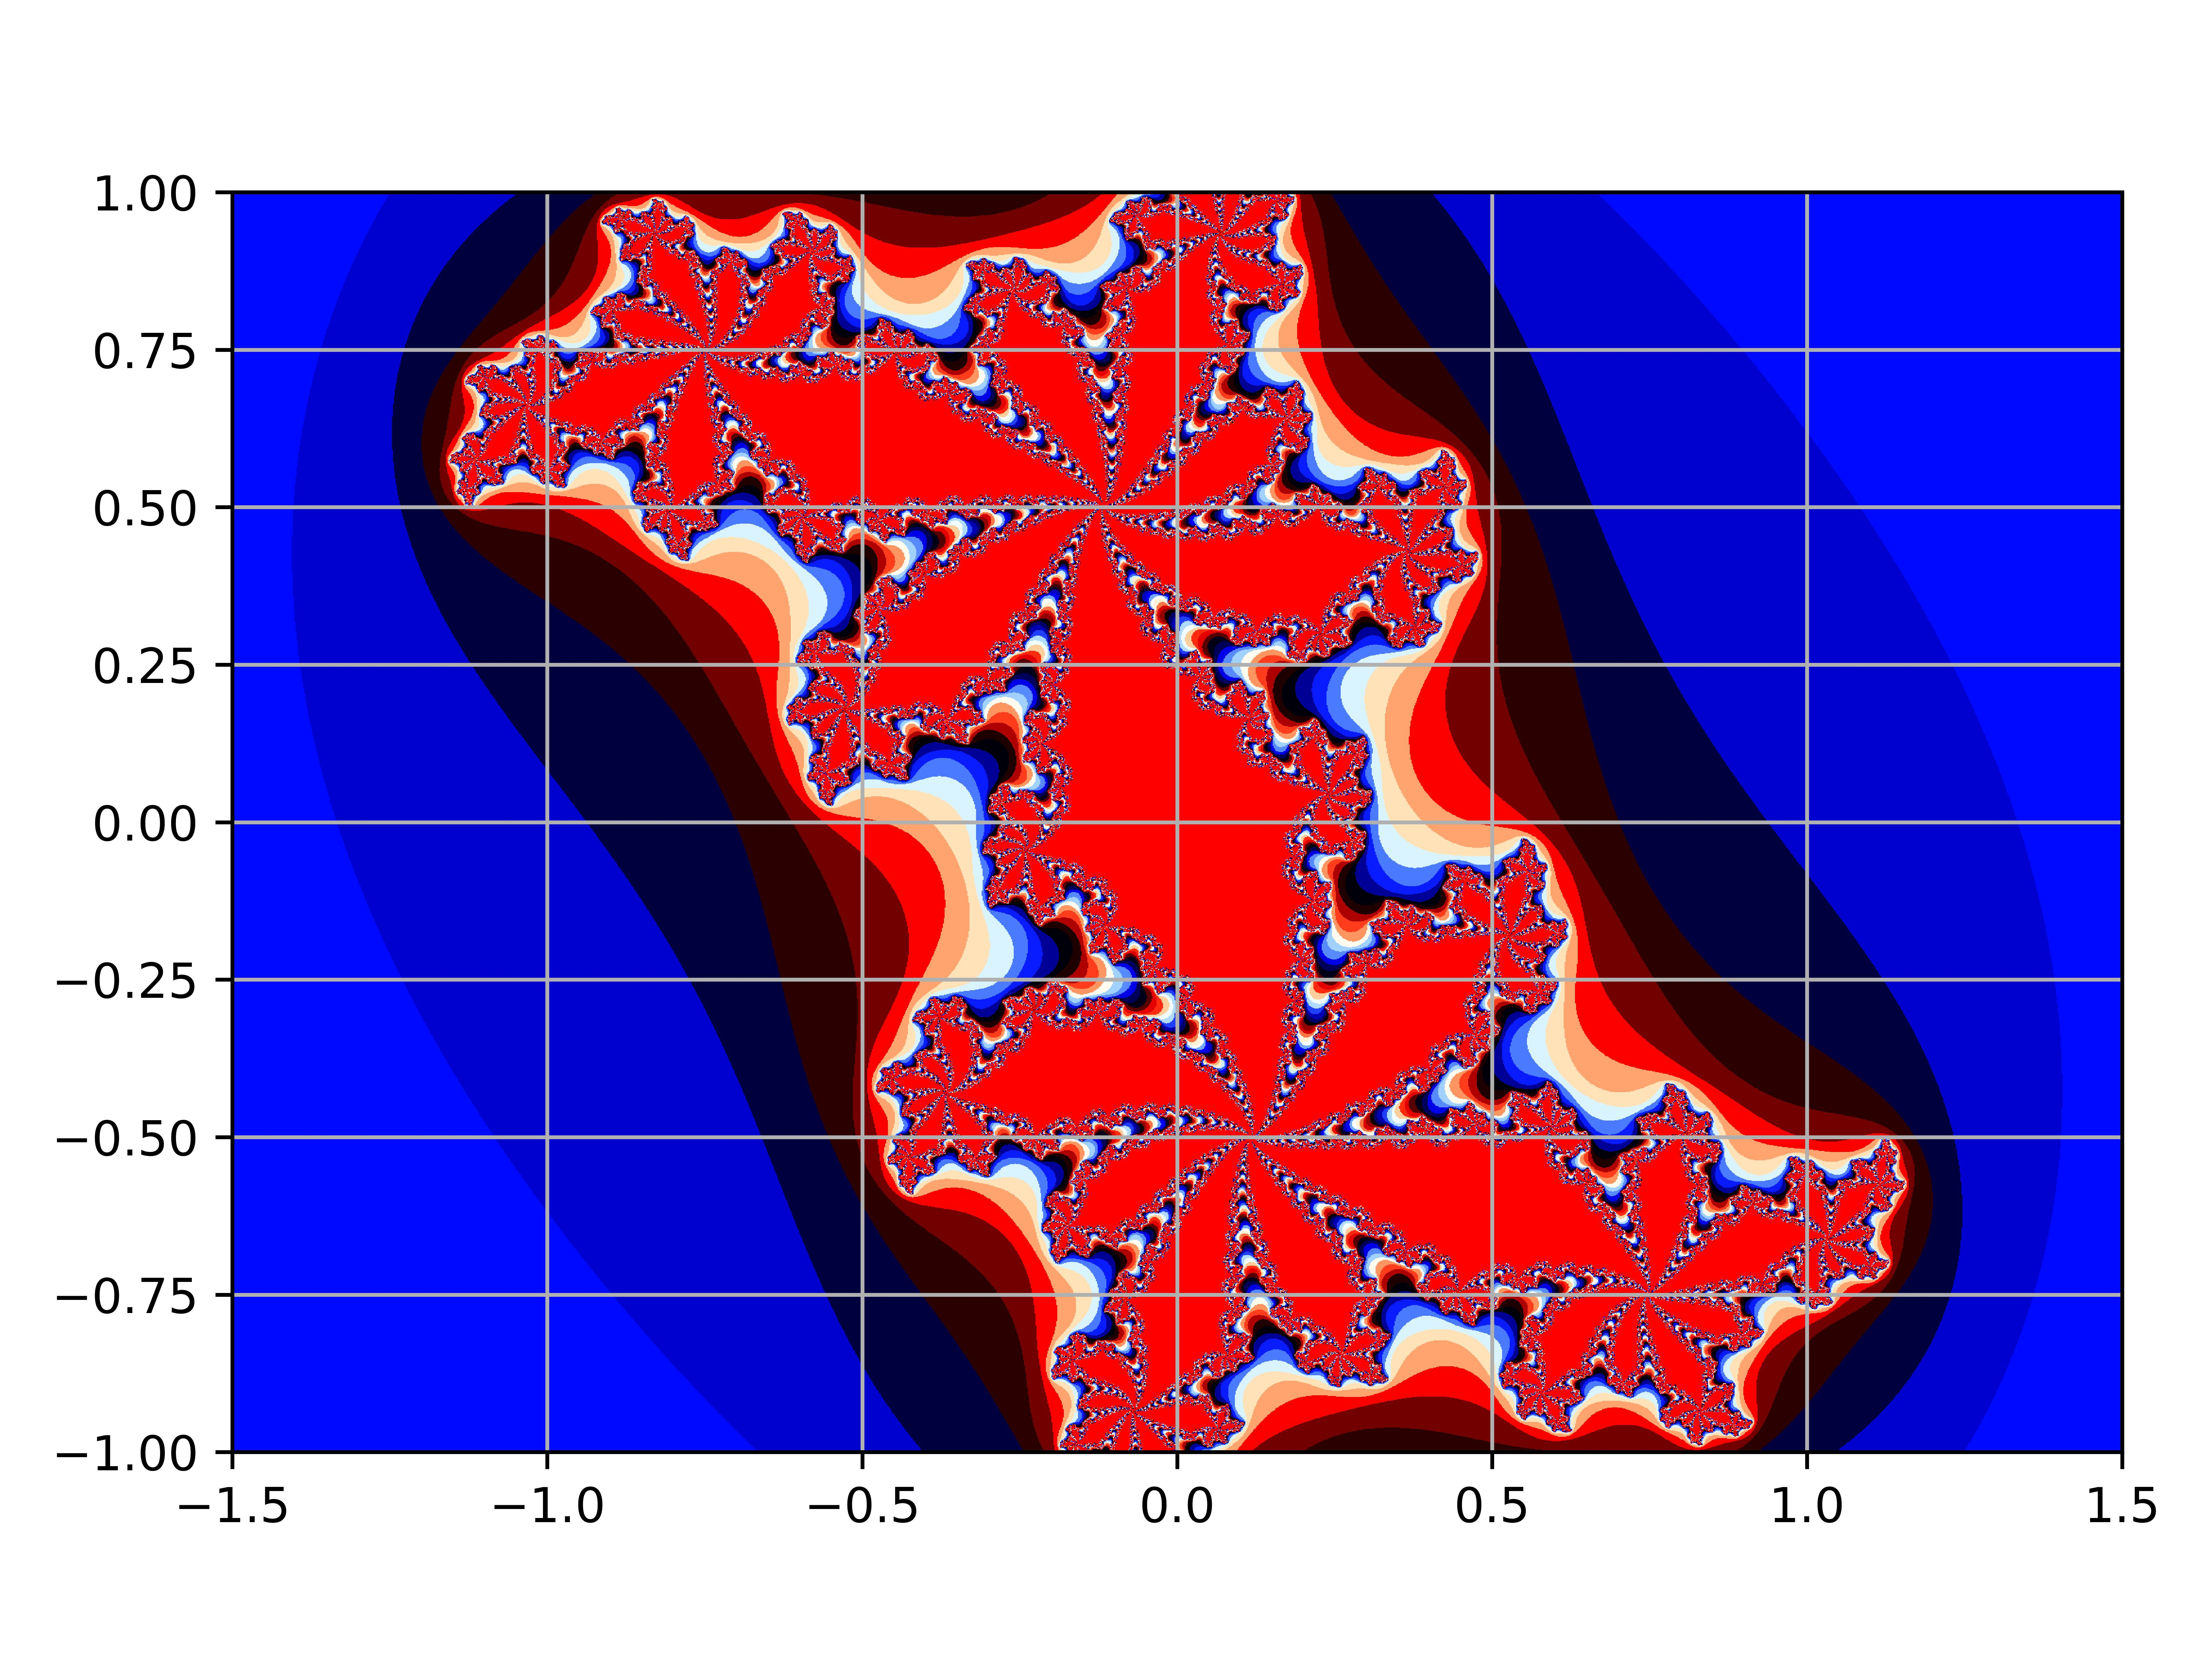
\includegraphics[width=\textwidth]{images/hw_10/julia_3.jpg}
    \caption{Множина Жулія з палітрою \texttt{gnuplot}. Тут взагалі не зрозуміло, що відбувається :)}
    \label{fig:3}
\end{figure}

\textbf{Множина Мандельброта.} Тут я також поекспериментував з палітрами та проміжками малювання. Результати нижче :)

\begin{figure}
    \centering
    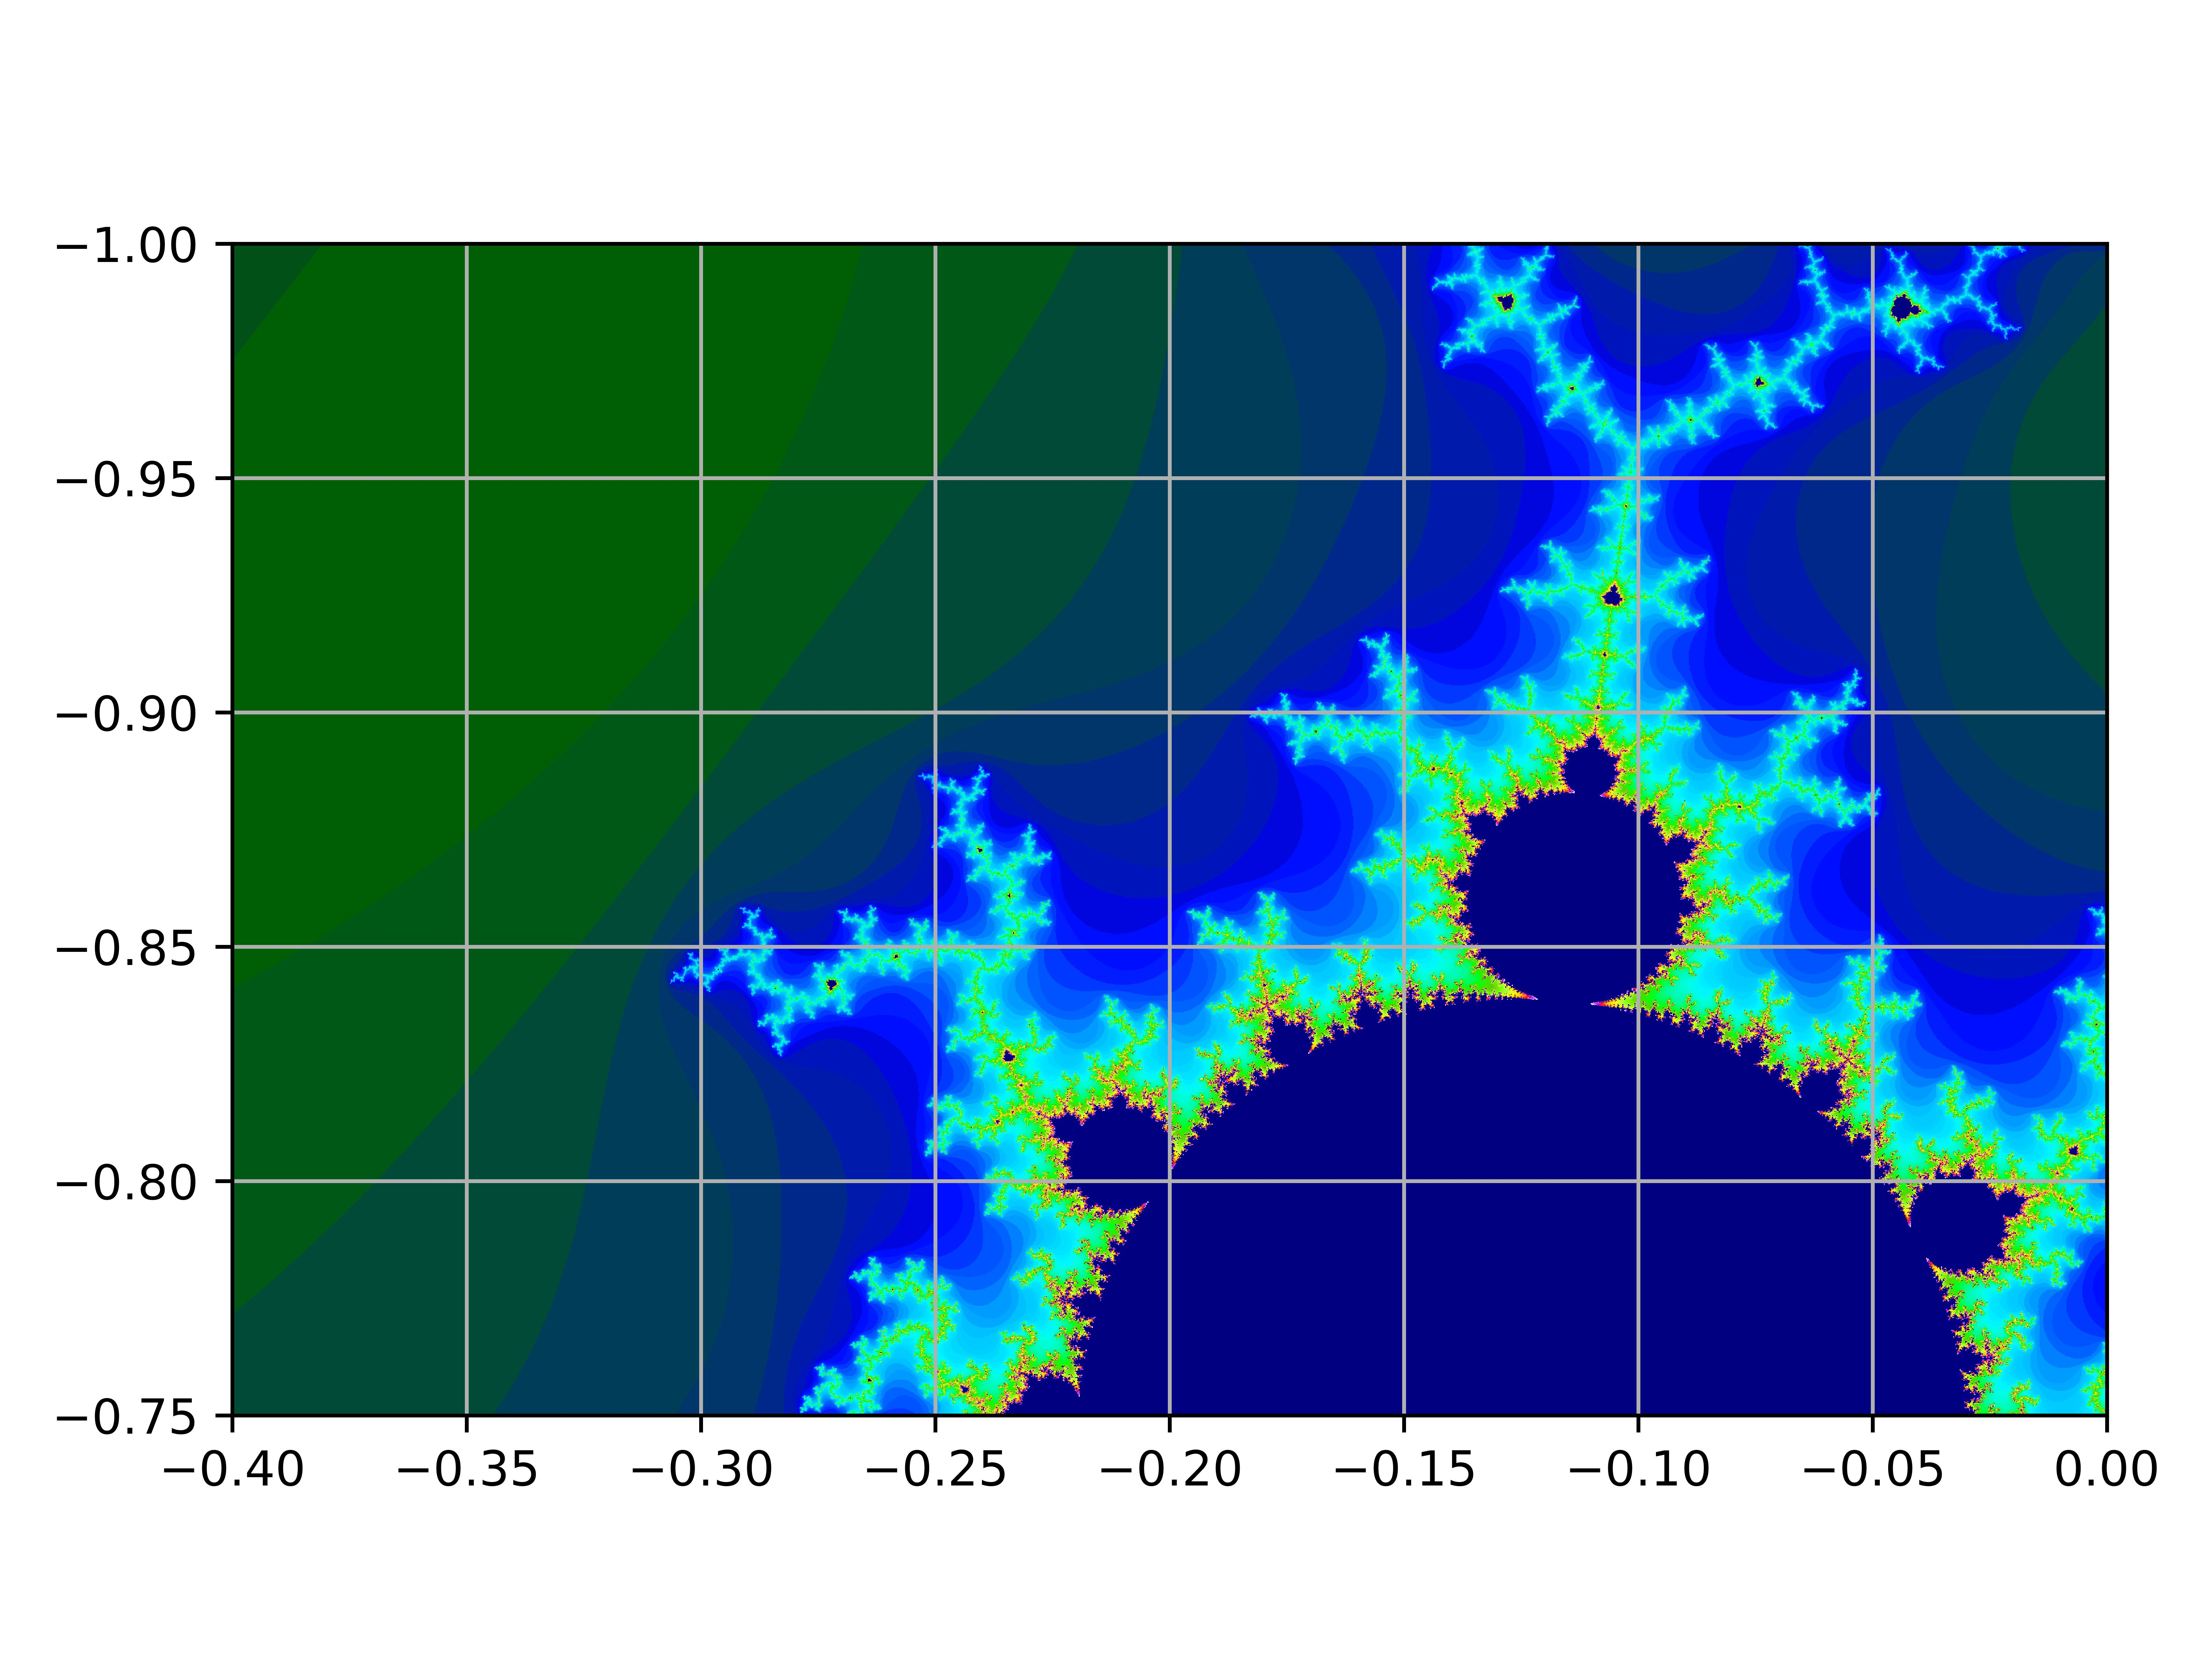
\includegraphics[width=\textwidth]{images/hw_10/mandelbrot_1.jpg}
    \caption{Множина Мандельброта з палітрою \texttt{gist\_ncar}. Цікаві земляні кольори :)}
    \label{fig:3}
\end{figure}

\begin{figure}
    \centering
    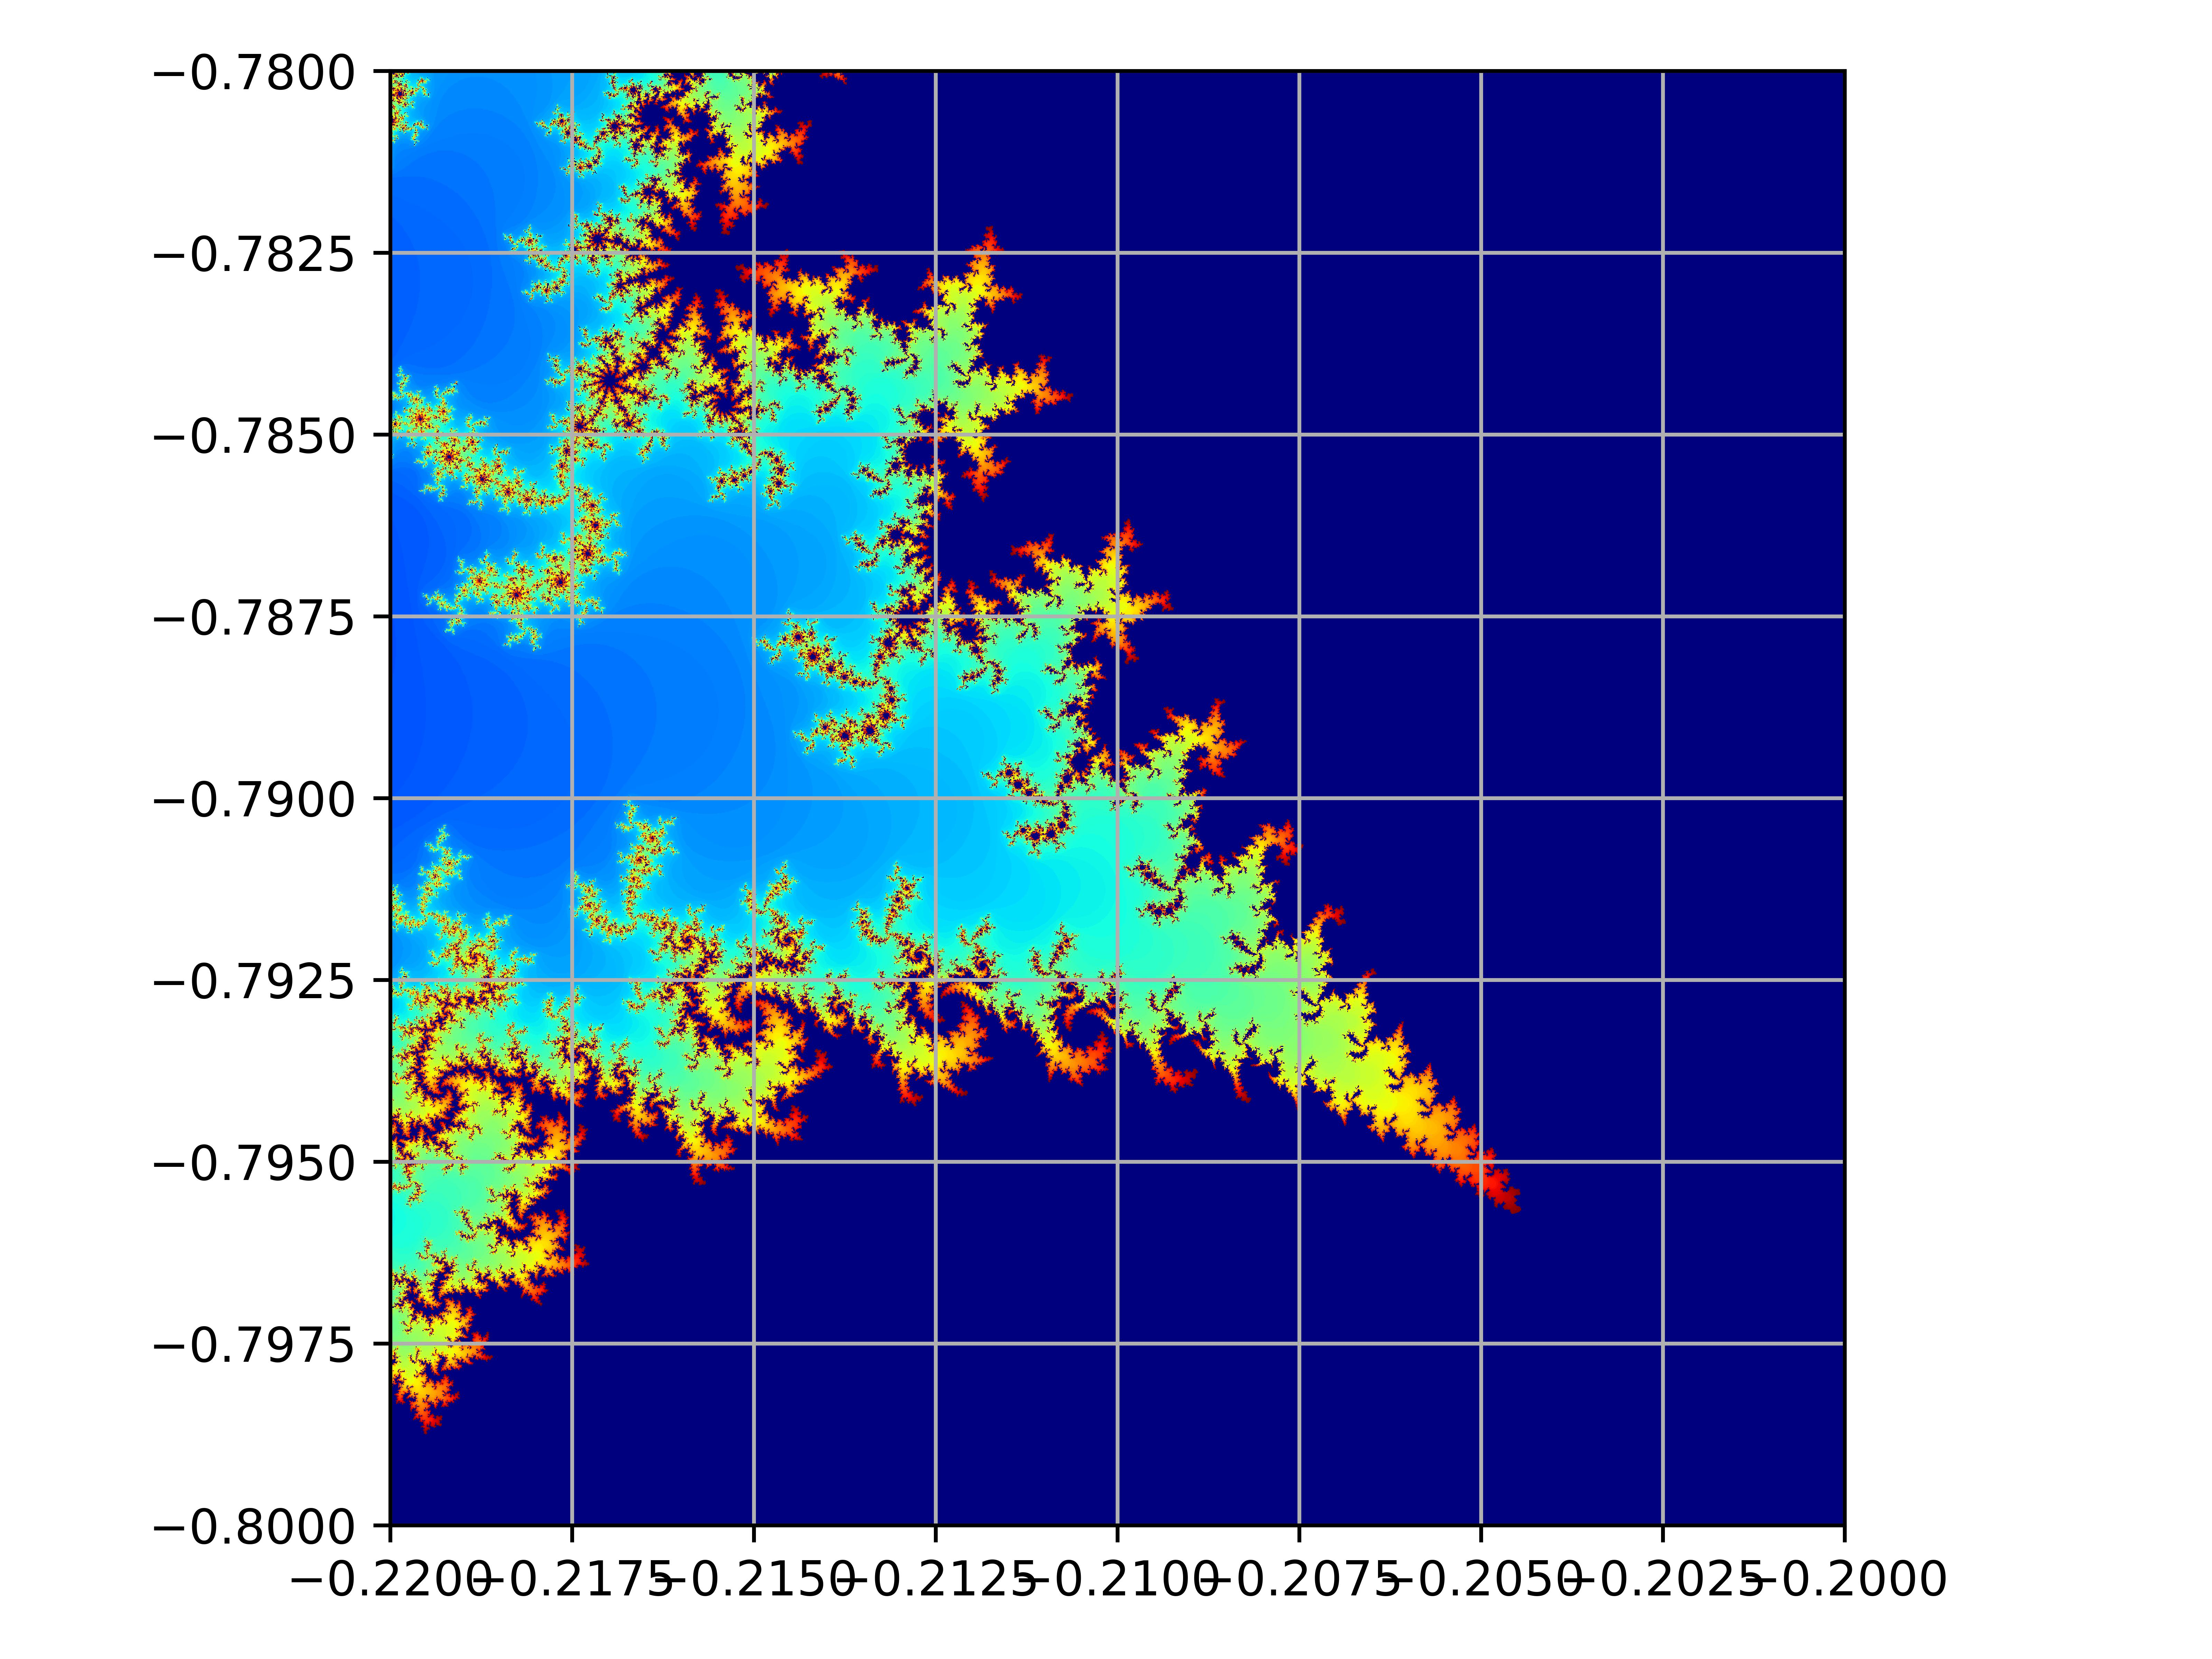
\includegraphics[width=\textwidth]{images/hw_10/mandelbrot_2.jpg}
    \caption{Множина Мандельброта з палітрою \texttt{jet}. Виглядає як берег острова :)}
    \label{fig:3}
\end{figure}

\begin{figure}
    \centering
    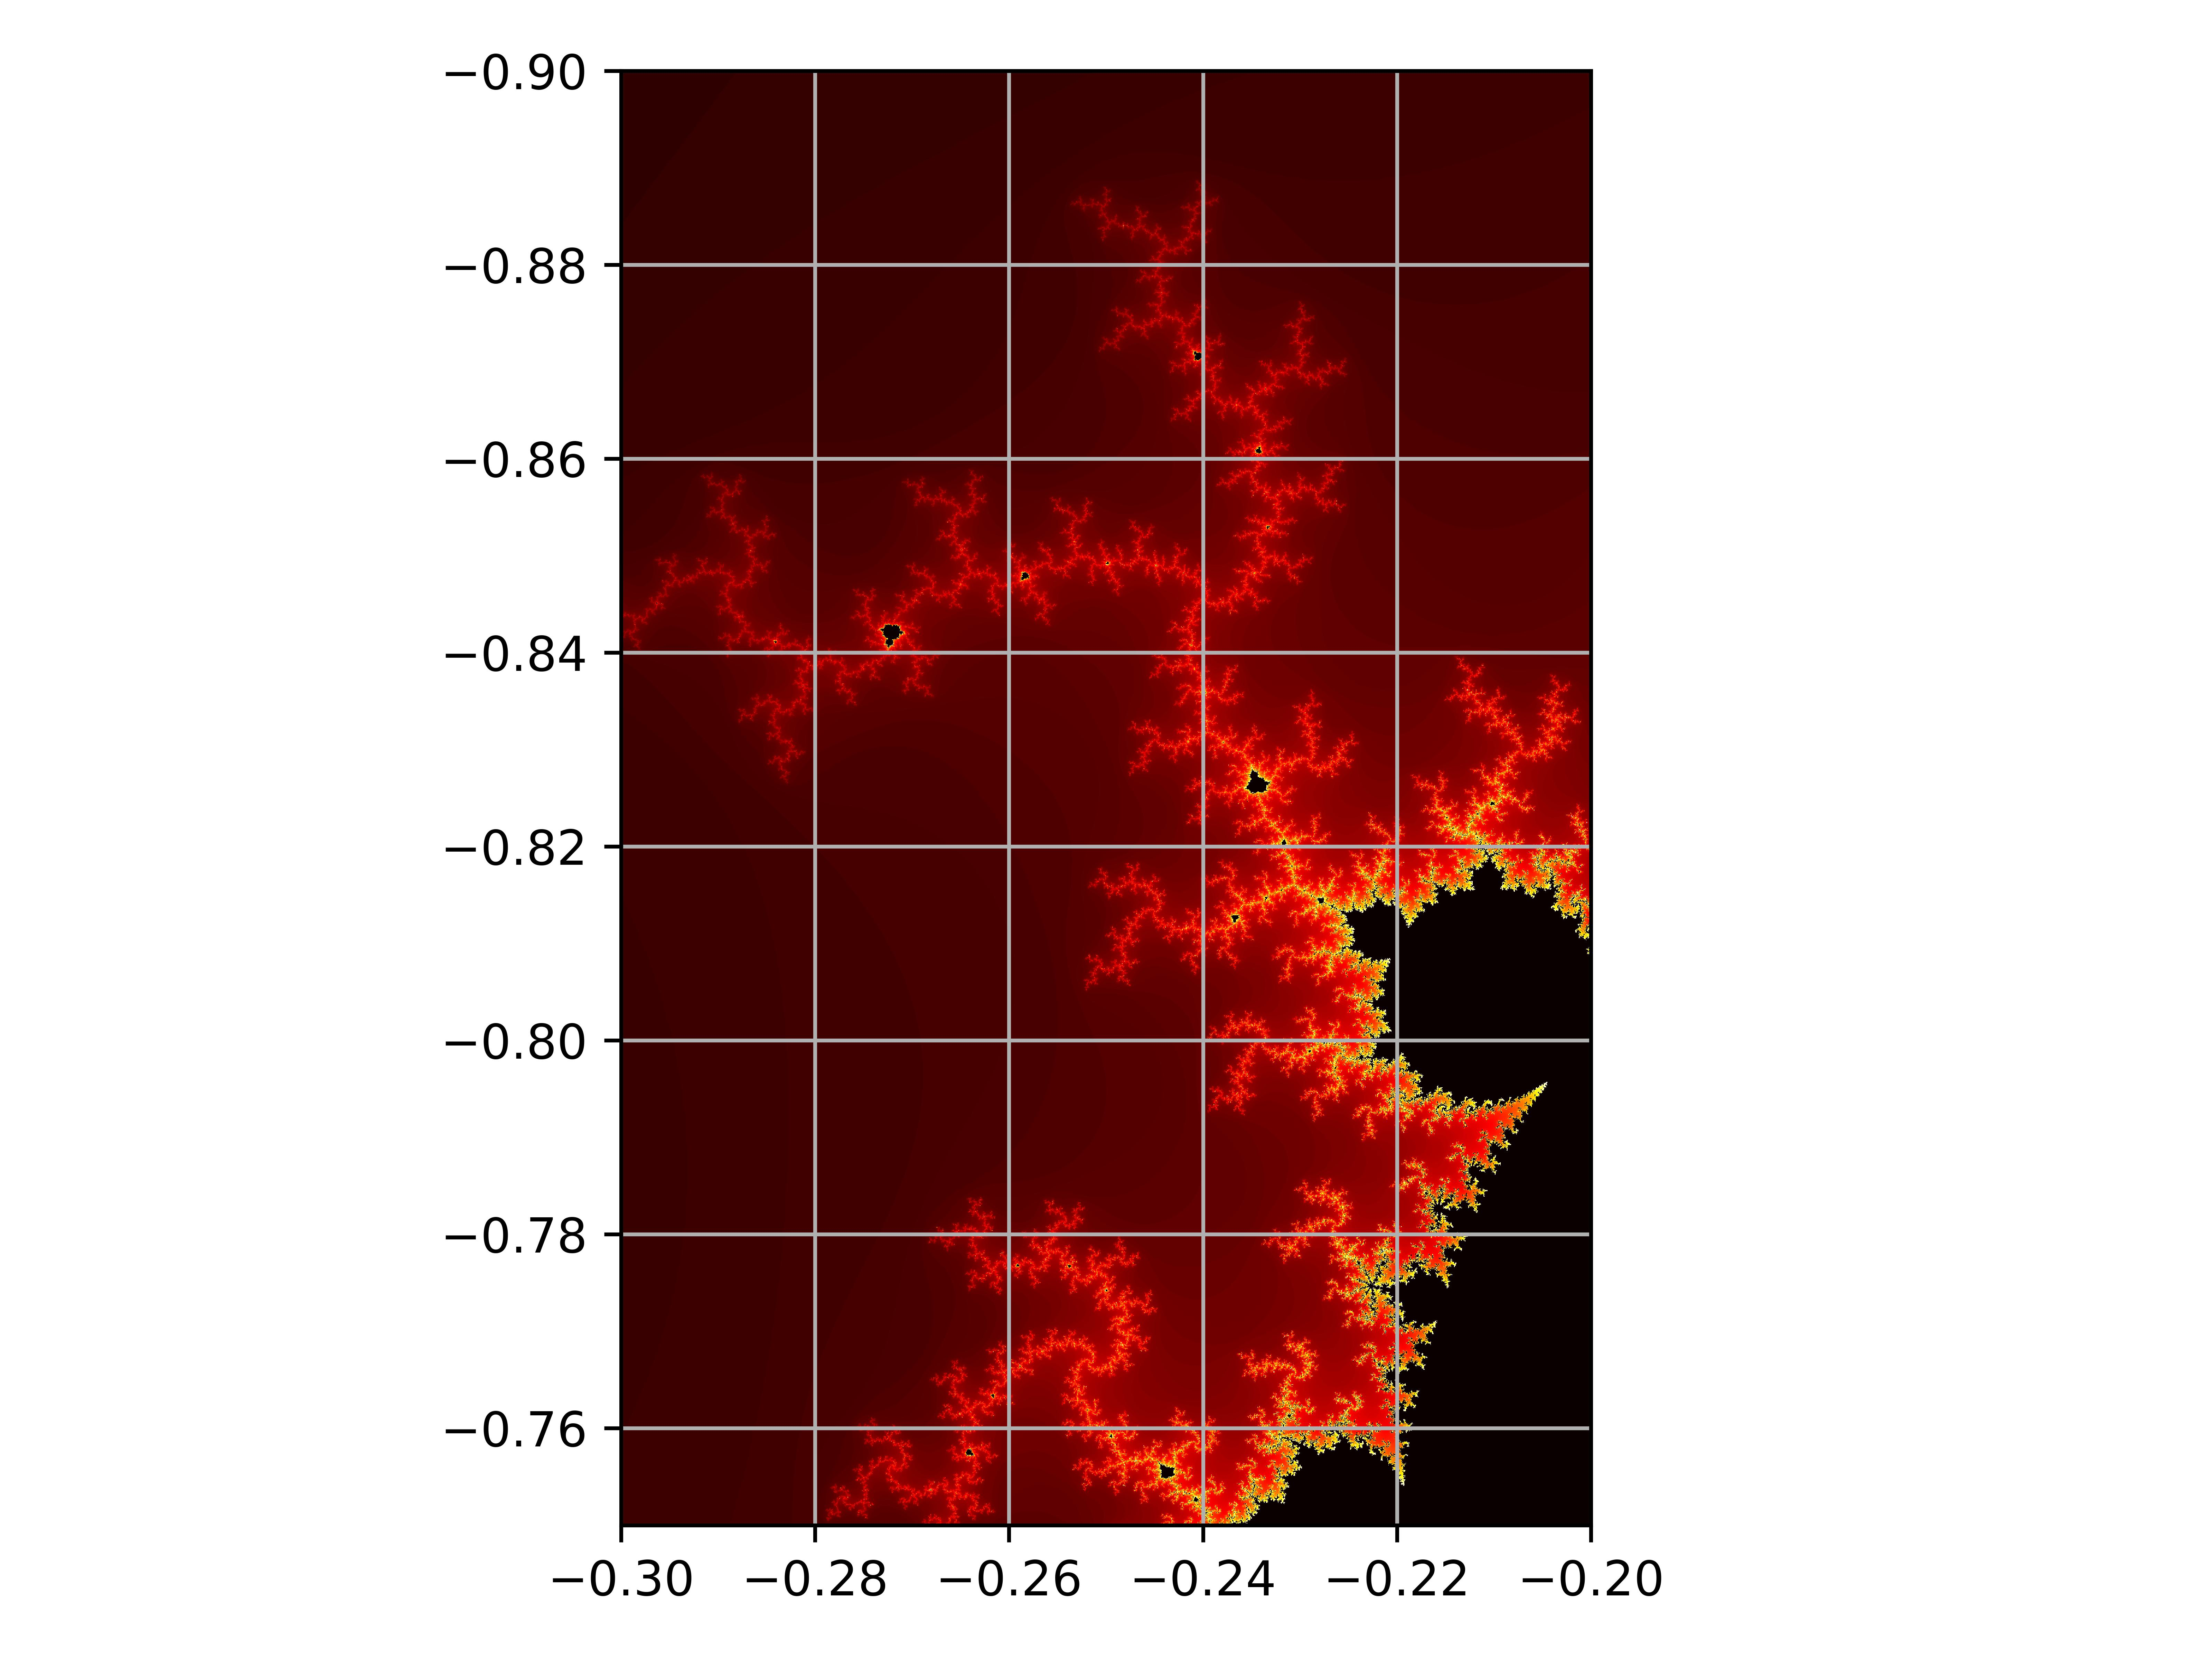
\includegraphics[width=\textwidth]{images/hw_10/mandelbrot_3.jpg}
    \caption{Множина Мандельброта з палітрою \texttt{hot}. Кольори лави :)}
    \label{fig:3}
\end{figure}

\end{document}
